% tocomputer (new_microarchitecture)
%
%\documentclass[10pt,dvips]{article}
%\documentclass[10pt,twocolumn]{article}
\documentclass[12pt]{slides}
\usepackage[english]{babel}
\usepackage{epsfig}
\usepackage{amssymb}
%\usepackage{fancyheadings}
%\usepackage[T1]{fontenc}
%\usepackage[latin1]{inputenc}
%\usepackage{twocolumn}
%\usepackage{verbatim,moreverb,doublespace}
%\usepackage{rotate,lscape,dcolumn,array,rotating,latexsym}
%
%\input{epsf}
%
% for somebody (I forget now !)
%\textwidth 175mm
%\textheight 225mm
%\topmargin -4.5mm
%
% for somebody else (I also forget now !)
%\textwidth 6.6in
%\textheight 239mm
%\topmargin -15mm
%\leftmargin -2.0in
%
% for IEEE (single-column format)
%\oddsidemargin 0mm
%\evensidemargin 0mm
%
% for IEEE (two-column format)
%\oddsidemargin 0mm
%\evensidemargin 0mm
%
%
%
\newtheorem{trans}{Transaction}
\newtheorem{snarf}{Snarfing Rule}
%
\begin{document}
%
% going to 1mm here recoups some good space ! :-)
%\parskip 1mm
\parskip 2mm
%
%
%
%
%

\begin{slide}
\begin{center}
\textbf {Resource-Flow Execution Model}
\end{center}
%
\begin{itemize}
%
\item Achieving high IPC
%
\item Exploit as much speculation as possible.  
%
\item Going beyond the traditional data and control flow dependency constraints 

\item Execution is based upon the need for an instruction to execute and
the availability of resources.  

\end{itemize}
\end{slide}




\begin{slide}
\begin{center}
\textbf {Time Tags}
\end{center}
%
\begin{itemize}
%

\item In the Resource-Flow execution model, instructions are executed
speculatively in an out-of-order fashion.  

\item Used enforce the correct data and control dependencies 

\item Small integer uniquely identifies the position of an instruction or an
operand in program ordered time with 

\end{itemize}
\end{slide}



\begin{slide}
\begin{center}
\textbf {Transactions}
\end{center}
%
\begin{itemize}
%
\item Communication between instructions is realized through a set of
transactions. 
%
\item
Two general froms: 
\begin{enumerate}
\item \emph{forward} 
\item \emph{backward}
\end{enumerate}
%
\item Each instruction has an associated data structure 

%
\end{itemize}
\end{slide}



\begin{slide}
\begin{center}
\textbf {Active Station Data Structure}
\end{center}
%
\begin{list}{\mbox{}}
\tiny{
\item $\mathbf{AS_i.en}$ is a binary value which is set if the Instruction is enabled
and its result is used in the execution of the program.
\item $\mathbf{AS_i.tt}$ holds the time-tag value.
\item $\mathbf{AS_i.op_x}$ where $x \in \{1,2,\ldots\}$ holds the input operands of
the instruction $I_i$ residing in the active station.
\item $\mathbf{AS_i.op_x.last\_tt}$ holds the source time-tag of the last snarfed
transaction that its data was used in the execution of the $I_i$.  Since each operand
can have a different source, a separate variable for each operand is needed.
\item $\mathbf{AS_i.D}$ is the address of the output operand of $I_i$.
\item $\mathbf{AS_i.D.data}$ is the value of the $AS_i.D$ operand.
\item $\mathbf{AS_i.mem.addr}$ holds the memory address (valid only if $I_i$ is
 a load or store instruction).
\item $\mathbf{AS_i.mem.data}$ holds the memory value (valid only if $I_i$ is a load
or store instruction).
\item $\mathbf{AS_i.mem.last\_tt}$ holds the source time-tag of the last memory
value that was snarfed. (valid only if $I_i$ is a load instruction).
\item $\mathbf{AS_i.D.last\_data}$ holds the output operand value produced by the
last enabled instruction before $I_i$.  In case $I_i$ is disabled, this value is
forwarded as the correct value of the destination register.
\item $\mathbf{AS_i.outcome}$ is a binary value set according to the outcome of the branch
(valid only if $I_i$ is a branch instruction).
\item $\mathbf{AS_i.target}$ holds the time-tag of the branch target instruction
(valid only if $I_i$ is a branch instruction).
\item $\mathbf{AS_i.CEP}$ structure holds the information regarding the Closest
Enabled Previous branch.
}
\end{list}

\end{slide}



\begin{slide}
\begin{center}
\textbf {Register Operations}
\end{center}
%
\begin{itemize}
%
\item 
Instruction operands: register, memory and predicate 
%
\end{itemize}

\begin{trans}
\mbox{} \\
\indent $fw.trans = RegVal $ \\
\indent $fw.tt = AS_i.tt$ \\
\indent $fw.op = AS_i.D $ \\
\indent $fw.data = AS_i.D.data $
%\flushright{$\diamondsuit$}
%\flushright{$\blacksquare$}
\end{trans}


\begin{trans}
\mbox{} \\
\indent $fw.trans = Relay$ \\
\indent $fw.tt = AS_i.tt$ \\
\indent $fw.op = AS_i.D $ \\
\indent $fw.data = AS_i.D.last\_data $
\end{trans}

\end{slide}

\begin{slide}
\begin{center}
\textbf {Snooping and Snarfing}
\end{center}
%
\begin{itemize}
%
\item Each AS snoops the bus for new operand values
%
\item A relevant operand value is consumed (snarfed)
%
\end{itemize}

\begin{snarf}
\label{snar:regop}
\mbox{} \\
\(
\begin{array}{ll}
(fw.trans = RegVal)\ \textup{or} \ (fw.trans = Relay) & \textup{and} \\
AS_i.op_x.last\_tt \leq fw.tt < AS_i.tt & \textup{and}\\
AS_i.op_x.addr = fw.op.addr \\
\hspace{3em} \Rightarrow \\
AS_i.op_x.last\_tt \leftarrow fw.tt\\
AS_i.op_x.data \leftarrow fw.data
\end{array}
\)
\end{snarf}



\begin{snarf}
\label{snar:outregop}
\mbox{} \\
\(
\begin{array}{ll}
(fw.trans = RegVal)\ \textup{or} \ (fw.trans = Relay) & \textup{and} \\
AS_i.op_x.last\_tt \leq fw.tt < AS_i.tt & \textup{and}\\
AS_i.D.addr = fw.op.addr \\
\hspace{3em} \Rightarrow \\
AS_i.D.last\_tt \leftarrow fw.tt\\
AS_i.D.last\_data \leftarrow fw.data
\end{array}
\)
\end{snarf}

\end{slide}



\begin{slide}
\begin{center}
\textbf {An Example}
\end{center}
%
%\begin{figure*}[th]
%\vspace{0.2 in}
%\setlength{\epsfxsize}{10cm}%7
%\centerline{\epsfbox{ttexec.eps}}
\centering
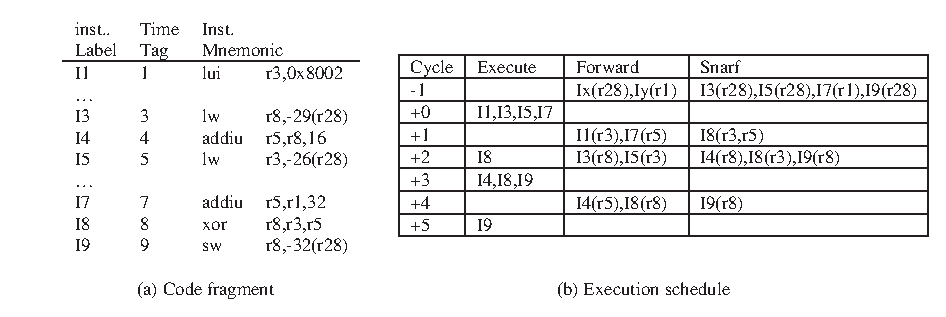
\epsfig{file=ttexec.eps,width=7.0in}
%\end{figure*}

\end{slide}



\begin{slide}
\begin{center}
\textbf {Hardware Predication}
\end{center}
%
\begin{itemize}
%
\item 
Predicated execution is an effective approach for handling conditional branches 
%
\item
In our microarchitecture predicates are generated at run-time.
%
\item
Each instruction computes its own enabling predicate by snooping 
predicate operands that are forwarded to it by earlier instructions 
%
\end{itemize}
\end{slide}



\begin{slide}
\begin{center}
\textbf {Hardware Predication}
\end{center}
%

%\begin{figure}
%\vspace{0.2 in}
%\setlength{\epsfxsize}{10cm}%7
%\centerline{\epsfbox{window.eps}}
%\centering
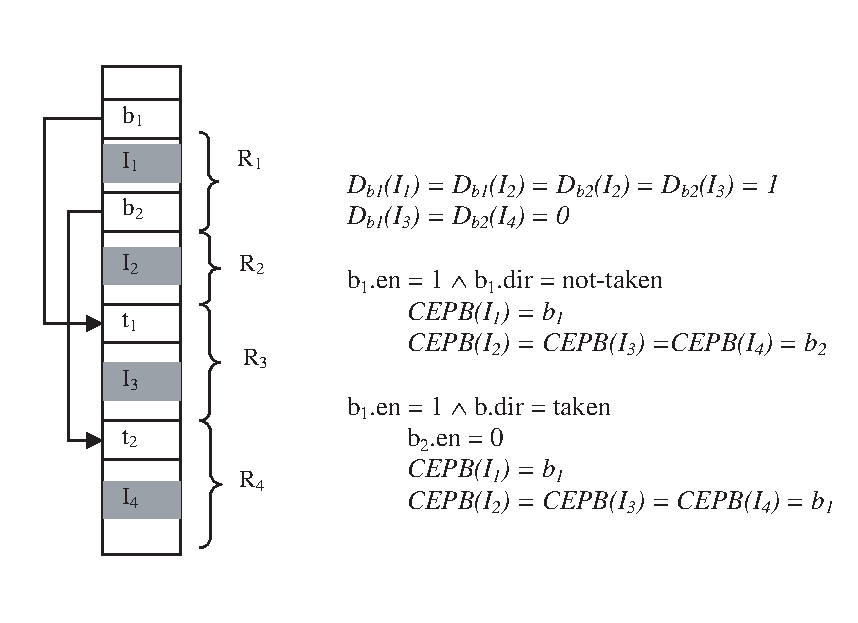
\epsfig{file=brdomain.eps,width=5.0in} 
%\end{figure}

\begin{list}{\mbox{}}
\small{
\item $T_b$: a binary value, set to one if the branch $b$ is
predicted taken
\item $en_j$: a binary value assigned to each
instruction $I_j$ and specifies whether the instruction is
executed or otherwise disabled.
\item $D_b(I_j $:] a binary value,
set to one if the instructions $I_j$ is in the domain of branch $b$.
\item $CEP(I_j $:] Closest Enabled Previous branch to instruction
$I_j$ in the static program-order.
}
\end{list}

Using the above definitions: 
\begin{equation}
\small{
\overline{en_j} = T_b \cdot D_b(I_j)  \textstyle{\ where\ } b = CEP(I_j)
}
\end{equation}
\end{slide}



\begin{slide}
\begin{center}
\textbf {Predication Transacions}
\end{center}
%
%

\begin{trans}
\mbox{} \\
\indent $fw.trans = PredVal $ \\
\indent $fw.tt = AS_i.tt$ \\
\indent $fw.dir = AS_i.outcome $ \\
\indent $fw.target = AS_i.target $
\end{trans}

\begin{trans}
 \mbox{} \\
 \indent $fw.trans = PredInv$ \\
 \indent $fw.tt = AS_i.tt$ \\
 \indent $fw.new\_tt = AS.CEP.tt $ \\
 \indent $fw.dir = AS_i.CEP.outcome $ \\
 \indent $fw.target = AS_i.CEP.target $
\end{trans}

\begin{snarf}
\label{snar:predval}
\mbox{} \\
\(
\begin{array}{ll}
(fw.trans = PredVal) \ \textup{or} \ (fw.trans = PredInv) & \textup{and} \\
AS_i.CEP.tt \leq fw.tt < AS_i.tt \\
\hspace{3em} \Rightarrow \\
AS_i.CEP.tt \leftarrow fw.tt\\
AS_i.CEP.outcome \leftarrow fw.outcome\\
AS_i.CEP.target \leftarrow fw.target
\end{array}
\)
\end{snarf}

\end{slide}



\begin{slide}
\begin{center}
\textbf {Harware Predication}
\end{center}
%

%\begin{figure}
%\vspace{0.2 in}
%\setlength{\epsfxsize}{10cm}%7
%\centerline{\epsfbox{window.eps}}
%\centering
\epsfig{file=dynpred.eps,width=7.0in}
%\end{figure}

\end{slide}



\begin{slide}
\begin{center}
\textbf {Memory Operations}
\end{center}
%
\begin{itemize}
%
\item 
Increasing number of instruction in flight means higher
probability that memory values generated by store operations will
be used by other load operations in the execution window
%
\item
Unlike register operands, the
architected address of a memory operand is not fixed.  
%
\end{itemize}

\begin{trans}
 \mbox{} \\
 \indent $fw.trans = MemVal$ \\
 \indent $fw.tt = AS_i.tt$ \\
 \indent $fw.mem.addr = AS_i.mem.addr $ \\
 \indent $fw.mem.data = AS_i.mem.data $
 \end{trans}


\begin{snarf}
\label{snar:memval}
\mbox{} \\
\(
\begin{array}{ll}
(fw.trans = MemVal) & \textup{and} \\
AS_i.mem.last\_tt \leq fw.tt < AS_i.tt & \textup{and}\\
AS_i.mem.addr = fw.mem.addr \\
\hspace{3em} \Rightarrow \\
AS_i.mem.last\_tt \leftarrow fw.tt\\
AS_i.mem.data \leftarrow fw.data
\end{array}
\)
\end{snarf}

\end{slide}


\begin{slide}
\begin{center}
\textbf {Memory Operations}
\end{center}
%
\begin{itemize}
%
\item 
The speculative nature of this microarchitecture could result in temporary incorrect
register values for the memory operations.
%
\item
It is necessary for a load to eventually
initiate a memory request using its resolved memory address.  
%
\item
Memory requests are sent
to both higher level memory and previous active stations.
%
\item
store operation with the same address in earlier
active stations will forward the memory value
%
\end{itemize}


\begin{trans}
\mbox{} \\
\indent $bw.trans = MemReq$ \\
\indent $bw.tt = AS_i.tt$ \\
\indent $bw.mem.addr = AS_i.mem.addr $
\end{trans}

\end{slide}



\begin{slide}
\begin{center}
\textbf {Memory Operations}
\end{center}
%
\begin{itemize}
%
\item 
A Disabled store operation needs to notify later loads
%
%
\end{itemize}

\begin{trans}
\mbox{} \\
\indent $fw.trans = MemNul$ \\
\indent $fw.tt = AS_i.tt$ \\
\end{trans}

\end{slide}



\begin{slide}
\begin{center}
\textbf {Summary of Operations}
\end{center}
%



%\begin{table}
\begin{center}
\tiny{
\begin{tabular}{|l|l||l|l|l|}
\hline Instruction & Snarfed & AS &
\multicolumn{2}{c|}{Transaction}\\ \cline{4-5}
Type & Data & Operation & enabled AS & disabled AS \\
\hline

 & a or b & execute & RegVal & - \\
 \emph{Register} & c & last\_c $\leftarrow$ c & - & -\\
 c $\leftarrow$ a \emph{op} b & en\_pred & - & - & RegVal \\
 & dis\_pred & - & Relay & - \\

 \hline

 & a & calc addr & MemReq & - \\
 \emph{Load} & M[a] & - & ReqVal & - \\
 r $\leftarrow$ M[a] & r & last\_r $\leftarrow$ r & - & -\\
 & en\_pred & - & - & RegVal \\
 & dis\_pred & - & Relay & - \\

 \hline

 & a & calc addr & MemNul & - \\
 \emph{Store} & r & - & MemVal & - \\
 M[a] $\leftarrow$ r & en\_pred & - & - & MemVal \\
 & dis\_pred & - & MemNul & - \\

 \hline

 & a or b & compare & PredVal & - \\
 \emph{Branch} & en\_pred & compare & - & PredVal \\
 br a,b,target & dis\_pred & - & PredInv & - \\

\hline
\end{tabular}
}
\end{center}
%\end{table}
%

\end{slide}

\end{document}
